\chapter{Work Breakdown}

\section{Project Schedule}

\begin{figure}[!ht]
\centering
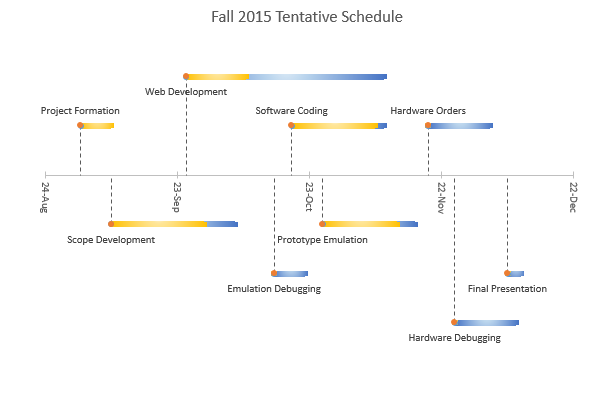
\includegraphics[scale=0.65]{./figures/fall-timeline}
\caption{Tentative Fall 2015 Project Schedule Overview}
\label{figure:fall-timeline}
\end{figure}

\begin{table}
\centering
\begin{tabular}{l  c  c  c}
Task & Start & Duration & End \\
\hline
Project Formation & 2015-09-01 & 7 & 2015-09-08 \\
Scope Development & 2015-09-08 & 28 & 2015-09-15 \\
Web Development & 2015-09-25 & 45 & 2015-10-02 \\
Emulation Debugging & 2015-10-15 & 7 & 2015-10-15 \\
Software Coding & 2015-10-16 & 21 & 2015-10-26 \\
Project Formation & 2015-10-26 & 21 & 2015-10-26 \\
Hardware Orders & 2015-11-19 & 14 & 2015-11-26 \\
Hardware Debugging & 2015-11-25 & 14 & 2015-12-2 \\
Final Presentation & 2015-12-7 & 3 & 2015-12-14 \\
\end{tabular}
\caption{Fall 2015 Detailed Project Schedule}
\label{table:risk}
\end{table}
\vspace{0.3cm}

\begin{figure}
\centering
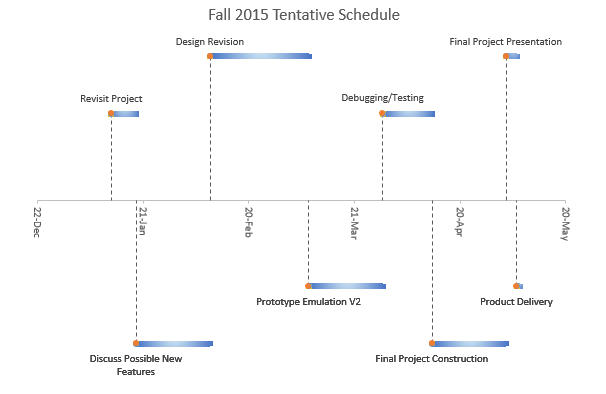
\includegraphics[scale=0.65]{./figures/spring-timeline}
\caption{Tentative Spring 2016 Project Schedule}
\label{figure:fall-timeline}
\end{figure}

\begin{table}
\centering
\begin{tabular}{l  c  c  c}
Task & Start & Duration & End \\
\hline
Revisit Project	& 2016-01-12 & 7 & 2016-01-19 \\
Discuss Possible New Features & 2016-01-19 & 21 & 2016-01-19 \\
Design Revision & 2016-02-09 & 28 & 2016-03-08 \\
Prototype Emulation V2 & 2016-03-08 & 21 & 2016-03-29 \\
Debugging/Testing & 2016-03-29 & 14 & 2016-04-12 \\
Final Project Construction & 2016-04-12 & 21 & 2016-05-03 \\
Final Project Presentation & 2016-05-03 & 3 & 2016-05-06 \\
Product Delivery & 2016-05-06 & 1 & 2016-05-07 \\
\end{tabular}
\caption{Spring 2016 Detailed Project Schedule}
\label{table:risk}
\end{table}
\vspace{0.3cm}


\section{Risks and Feasability Assessment}

This project is routinely implemented in industry with high success rates. Several software implementations of SCADA honeypots already exist in the open source community. However, our implementation will be custom because the client has a secondary goal of including an IDS on the system. Creating the honeypot software from scratch will minimize the resources required from the platform. This is important because the computer needs to be a small standalone device. A Raspberry PI only has 512MB of RAM for example and an IDS typically uses a lot of memory and process cycles. Most risk can be mitigated with proper contingency planning, as summarized in Table \ref{table:risk}.


\vspace{0.5cm}
\begin{table}[h]
\centering
\begin{tabular}{l  c  r}
Component & Risk & Contigency Plan \\
\hline
Web Server Honeypot & Low & Utilize open source nginx\footnotemark \\
SSH Server Honeypot & Low & Use open source Kippo SSH\footnotemark \\
Event Alerts & Medium & Switch from REST API to SMTP \\
SCADA Honepot & Medium & Use open source Conpot\footnotemark \\
Intrusion Detection System & High &  Use IPTables Logging \\
\end{tabular}
\caption{Summary of project components and implementation risk}
\label{table:risk}
\end{table}
\vspace{0.3cm}

% handle footnotes in table
\addtocounter{footnote}{-1}
\footnotetext{\url{https://www.nginx.com}}

\addtocounter{footnote}{1}
\footnotetext{\url{https://github.com/desaster/kippo}}

\addtocounter{footnote}{1}
\footnotetext{\url{http://conpot.org/}}

Installing an IDS on a small platform such as a Raspberry PI may not be feasible. If this is the case, developing a custom platform with greater processing power and more memory will be explored. If this isn't feasible, then the secondary goal will have to be canceled. However, the overall honeypot implementation carries a low risk of failure.

\section{Cost Considerations}

Alliant Energy requires service in twenty eight different locations. Each location will house a standalone minimal computer. At this stage of development, the Raspberry PI is the assumed device. A model description is listed in Table \ref{table:cost}.

\vspace{0.5cm}
\begin{table}[h]
\centering
\begin{tabular}{l l l l}
Model & Unit Cost & Vendor & Total Cost \\
\hline
Raspberry PI B+ & \$30 Plus Tax & Allied Electronics & \$840 Plus Tax \\
\end{tabular}
\caption{Summary of implementation costs}
\label{table:cost}
\end{table}
\vspace{0.5cm}

This device is subject to change throughout the project development depending on implementation and client needs. However, as of the present date, the Raspberry PI is the best known device. An updated version of the plan may be submitted if a better hardware implementation is found. This cost analysis reflects an initial estimate. It does not reflect future maintenance cost.
